%%% Reusable Start
\documentclass[a4paper,4pt]{article}
\usepackage[UTF8]{ctex}
\usepackage{geometry}
\usepackage{titlesec}
\usepackage{indentfirst}
\usepackage{graphicx} %use graph format
\usepackage{subfigure}
\usepackage{epstopdf}
\usepackage{hyperref}
\usepackage{float}
\usepackage{amsmath}
\usepackage{amssymb}
\usepackage{multirow}
\usepackage{array}
\usepackage{enumerate}
\usepackage{enumitem} 
\usepackage{bookmark}
\usepackage{booktabs}
\usepackage{multirow}
\usepackage{bigstrut}
\usepackage[backend=bibtex]{biblatex}
\usepackage{pgfplots}
\usepackage{pgfplotstable}
\usepackage{siunitx}
\usepackage{datetime}
%插入中文日期
\renewcommand{\today}{\number\year 年 \number\month 月 \number\day 日}
%% for inserting code
\usepackage{listings}
\usepackage{xcolor}
\definecolor{mygreen}{rgb}{0.3,0.7,0}  
\definecolor{mygray}{rgb}{0.5,0.5,0.5}  
\definecolor{myblue}{rgb}{0.4,0.7,1}
\definecolor{mywhite}{rgb}{0.9,0.9,0.9}
\definecolor{mymauve}{rgb}{0.58,0,0.82}
\definecolor{mybackcolor}{RGB}{62,62,62}
\definecolor{myIdt}{rgb}{0.8,0.6,1}
\lstset{ %  
  backgroundcolor=\color{mybackcolor},   % choose the background color; you must add \usepackage{color} or \usepackage{xcolor}  
  basicstyle=\small\ttfamily\color{mywhite},        % the size of the fonts that are used for the code  
  breakatwhitespace=false,         % sets if automatic breaks should only happen at whitespace  
	breaklines=true,                 % sets automatic line breaking  
  captionpos=bl,                    % sets the caption-position to bottom  
  commentstyle=\color{mygreen},    % comment style  
  %deletekeywords={...},            % if you want to delete keywords from the given language  
  escapeinside={\%*}{*)},          % if you want to add LaTeX within your code  
  extendedchars=true,              % lets you use non-ASCII characters; for 8-bits encodings only, does not work with UTF-8  
  %frame=single,                    % adds a frame around the code  
  keepspaces=true,                 % keeps spaces in text, useful for keeping indentation of code (possibly needs columns=flexible)  
  keywordstyle=\color{myblue},       % keyword style  
  %language=Python,                 % the language of the code  
  morekeywords={*,...},            % if you want to add more keywords to the set  
  numbers=left,                    % where to put the line-numbers; possible values are (none, left, right)  
  numbersep=-15pt,                   % how far the line-numbers are from the code  
  numberstyle=\small\color{mygray}\ttfamily, % the style that is used for the line-numbers  
  rulecolor=\color{black},         % if not set, the frame-color may be changed on line-breaks within not-black text (e.g. comments (green here))  
  showspaces=false,                % show spaces everywhere adding particular underscores; it overrides 'showstringspaces'  
  showstringspaces=false,          % underline spaces within strings only  
  showtabs=false,                  % show tabs within strings adding particular underscores  
  stepnumber=1,                    % the step between two line-numbers. If it's 1, each line will be numbered  
  stringstyle=\color{orange},     % string literal style  
  tabsize=2,                       % sets default tabsize to 2 spaces  
  %title=myPython.py                   % show the filename of files included with \lstinputlisting; also try caption instead of title  
	rulesepcolor=\color{red!20!green!20!blue!20},
	identifierstyle=\color{myIdt},
	} 
%% end of code style



\begin{document}

%第二种封面
\begin{titlepage}
	\heiti
	\vspace*{64pt}
	\begin{center}
		\fontsize{43pt}{0} \textbf{FC18参赛规则}\\
		\vspace*{36pt}
		\fontsize{43pt}{0}{内测版}\\
		\vspace*{280pt}
		\Large
		\rmfamily
		\begin{tabular}{lr} %表格,lr表示左对齐|右对齐
			\textbf{开发者}   & 自动化系科协竞赛部 \\
			\textbf{比赛网址} & ?                 \\
			\textbf{更新日期} & \today             \\
		\end{tabular}
	\end{center}
\end{titlepage}


\tableofcontents%目录
\newpage%换页

FC18为四方势力在地图上进行回合制对战的策略游戏,玩家需要力求攻占其他玩家的塔、占领尽可能大的领地、消灭或俘虏其他玩家的兵团以获得胜利。每个玩家需要编写AI,根据裁判程序提供的场地信息,决策己方势力在该回合的行动,并返回给裁判程序,以控制己方的行为。
\section{游戏说明}
作为塔防游戏,每个势力在开始时各在一角拥有一座塔,塔周围的一定区域是自己的领地。玩家需要利用塔的生产力,完成生产兵团或升级塔的任务。生产出的作战兵团可以在场上移动,攻击其他势力的塔或兵团(减少他们的生命值);生产出的工程兵团则可以完成修改地形、修理塔(恢复塔的生命值)的任务。其中,塔的等级越高,就会拥有更高的生产力、战斗力、生命值上限。塔也可以攻击敌方的兵团,如果塔内有己方兵团驻扎,则塔的战斗力会更强。

\section{角色说明}
游戏中有以下角色:塔$Tower$,作战兵团(分为战士$Warrior$、弓箭手$Archer$、法师),工程兵团(分为建设者$Builder$、开拓者$Extender$)。
\subsection{塔}
\subsubsection{概述}
塔是在地图上固定的,具有对一定范围内(距离为2及以内,即5*5的方形内)敌对势力塔或兵团自动攻击能力的建筑,每个势力最初时拥有1座塔,每个地图方格内最多有1座塔,每个势力最多拥有10座塔。当某势力没有塔时,该势力将被判为失败。地图上每个方格都有属于每个势力的占有属性值。每回合都将进行方格所属势力的判定,方格将属于4个势力中对该方格占有属性最高的一方。占有属性值由修建防御塔产生。防御塔可向周围地图附加己方的占有属性值,该属性值随着与防御塔距离的增加而衰减,并在5格外衰减为0,具体数据见表\ref{领地}。若有2方占有属性值同为最高,则该方格判定为过渡区域,过渡区域不允许建筑防御塔。
\begin{figure}[htbp]   %用htbp表示插入位置自动排版
	\centering
	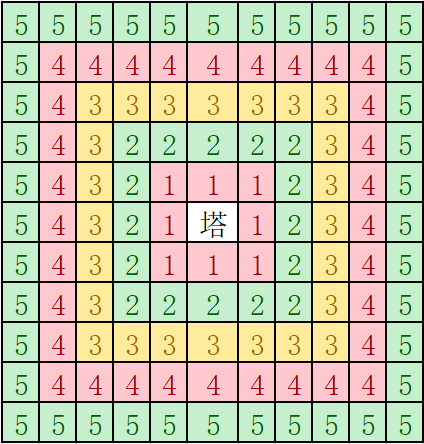
\includegraphics[width=2.5 in]{距离.png}
	\caption{距离计算示意图}
	\label{jpg:示例图片2}
\end{figure}

% Table generated by Excel2LaTeX from sheet 'Sheet1'
\begin{table}[htbp]
	\centering
	\caption{塔周围领地占有值}
	\begin{tabular}{c|c|c|c|c|c|c|c}
		\hline
		距防御塔距离d  & 0     & 1   & 2  & 3  & 4  & 5  & 6+ \bigstrut \\
		\hline
		施加占有属性值 & $inf$ & 100 & 80 & 50 & 20 & 10 & 0 \bigstrut  \\
		\hline
	\end{tabular}%
	\label{领地}%
\end{table}%


塔有以下属性:
\begin{enumerate}[fullwidth, itemindent=2em, label=(\arabic*)]
	\item 等级$N$。
	\item 生产力$W_N$。
	\item 等级生命力上限$HP_N$,当前生命力$hp$。
	\item 等级战斗力$F_N$,实际战斗力$f$。%TODO
	      \begin{lstlisting}[language={C++},title={防御塔结构体}]  %插入代码块
  	//@@@【FC18】防御塔结构体,有需要的信息再加
  	
  	struct TowerInfo {
  		
  		TTowerID      ID;   //防御塔ID
  		TPlayerID     ownerID;  //所属玩家ID
  		TPoint        position;    //位置
  		TProductPoint productPoint;  //生产力
  		TProductPoint productConsume;  //当前生产任务尚需完成的剩余生产力值
  		TBattlePoint  battlePoint;   //战斗力
  		THealthPoint  healthPoint;   //生命值
  		TLevel        level;       //等级
  		productType   pdtType;    //当前生产任务类型
  	};
  \end{lstlisting}

\end{enumerate}
\subsubsection{具体说明}
1)塔的等级$N$为1-8的正整数,从等级$N$升级到$N+1$需要消耗的生产力值为$40 \cdot N$。\par
2)塔会根据自身的等级状况获得一个生产力数值$W_N$,代表其一个回合能产生的生产力,具体的数据如表\ref{塔等级表}所示。生产力$W_N$每回合更新,如果该回合没有使用生产力,下一回合不会累积。在同一时刻,塔可以选择一种生产任务(包括生产战士、生产弓箭手、生产法师、生产建造者、生产开拓者、升级塔自身)每一种任务需要消耗不同的生产力点数,具体情况见表\ref{塔生产}。兵团生产任务完成之后,塔所在的方格将立即生成一个对应兵团。防御塔所在方格内允许存在多个兵团,不必遵循同一单元格仅能存在一个兵团的限制。在struct\ TowerInfo中,可以访问到该塔当前未完成的生产任务productType\ pdtType;和该任务有待完成的工作余量TProductPoint\ productConsume;\par
3)等级生命力上限$HP_N$仅与等级正相关,具体的数据如表\ref{塔等级表}所示。实际生命力$hp$会受到进攻而减小(具体结算方式如式\ref{hp1}和式\ref{hp2}所示)、由于建设者的维护而增加。当实际生命力$hp$被进攻方降低至0以下时,对方获得5分的击杀分,我方丧失该塔,塔等级下降4级:等级下降后,若不足1级,则塔消失,该单位恢复原来地形;若塔尚存在,则降级后的塔主权归对方所有(塔被俘虏)。\par
4)实际战斗力$f$为战斗中的战斗力。$f$是$F_N$、当前生命值$hp$、等级生命值上限$HP_N$、兵团驻扎情况带来战斗力增益$f_c$(具体增益规则如表\ref{兵团}所示)的函数。具体计算方法如下:

\begin{equation}
	f = F_N \cdot \frac{hp}{HP_N} + \Sigma f_b\label{f}
\end{equation}
兵团攻击塔时,生命值的结算方式如下:
\begin{equation}
	\begin{aligned}
		hp_{\text{塔}}   & \ -= & \ 30 \cdot k_c \cdot e^{0.04(f_{\text{兵}}-f_{\text{塔}})} & ;                       \\
		hp_{\text{兵团}} & \ -= & \ 28 \cdot e^{0.04(f_{\text{塔}}-f_{\text{兵}})}           & , \text{当兵团非弓箭手} \\
		hp_{\text{兵团}} & \ -= & \ 0                                                        & , \text{当兵团为弓箭手} \\
	\end{aligned}
	\label{hp1}
\end{equation}
塔只能攻击距离为2及以内的兵团。塔攻击兵团时,生命值的结算方式如下:
\begin{equation}
	\begin{aligned}
		hp_{\text{兵团}} & \ -=\ 30 \cdot e^{0.04(f_{\text{塔}}-f_{\text{兵}})}, \text{对于所有兵团种类} \\
		hp_{\text{塔}}   & \ -=\ 0                                                                       \\
	\end{aligned}
	\label{hp2}
\end{equation}
\par
5)兵团驻扎(无需给兵团添加过驻扎到塔的命令,只要兵团在塔的位置,自动判定为驻扎)到塔,则被塔护卫。如果兵团驻扎到塔,则对该兵团发起的进攻会与塔结算,而不是与该兵团。但是,如果进攻发起方是防御塔,服从之前的规则,不存在塔与塔结算这一说,这次攻击兵团判定失败(塔不可以攻击驻扎在别人塔中的兵团)。具体见\ref{细则}。\par

你可以为塔添加以下操作:
\begin{enumerate}[fullwidth, itemindent=2em, label=(\arabic*)]
	\item 生产:在命令中指定命令类型为塔命令,塔操作类型为生产,塔ID,塔生产任务类型( <enum  productType> )。
	\item 攻击:在命令中指定命令类型为塔类型,塔操作类型为攻击,塔ID,塔的攻击对象序号,即可指定某一做塔攻击某一个对象。
\end{enumerate}
另外,请注意:
\begin{enumerate}[fullwidth, itemindent=2em, label=(\arabic*)]
	\item 每回合,每座塔最多可以添加一个操作。如果该回合玩家给一个塔添加了多个操作,则第二个及以后的操作会被自动忽略,且占用50个操作的余额(相当于填了废志愿),所以请不要添加大于一个操作。
	\item 如果你的操作是无效操作,则也不会起任何作用。无效操作包括试图攻击自己的对象、试图攻击超出攻击范围的对象、不存在对应序号的对象等。
	\item 如果上一回合塔选择了生产,但未完成该生产任务,本回合选择攻击,则上一回合的生产进度会被保留,这样在下一回合假如继续添加生产该任务的命令,会在上一回合基础上继续生产。
	\item 若防御塔的某个生产任务尚未完成,玩家又指定了新任务,则未完成的生产任务的完成度将被缓存起来,然后进行新的任务。之后再选择有一定完成度的任务的时候,只需要完成未完成的部分,即完成剩余的生产力消耗值。即如果上一回合塔选择了生产任务A,但未完成该生产任务A,本回合选择生产任务B,则上一回合的生产进度也会被保留,这样在下一回合假如继续添加生产任务A的命令,会在上一回合基础上继续生产。但是,由于接口所限,你只能通过TowerInfo访问到最近一次尚未完成的任务类型和余量,所以我们推荐一旦开始一种生产任务,中途不要切换别的生产任务(虽然你仍可以正常地生产它们)。
\end{enumerate}
\subsection{作战兵团}
在同一个时间,同一个地图方格(防御塔所在方格除外)内的作战兵团、工程兵团数量各自不能超过1个。当某个方格内同时存在一个势力的一个作战兵团和工程兵团,则称工程兵团被作战兵团护卫。任何战斗,都优先与作战兵团结算。若在某次战斗中,该护卫队中的作战兵团阵亡。此时进行一次判定,若敌方作战兵团也在作战中阵亡,则护卫队中的工程兵团仍属于原来的玩家;若敌方作战兵团未阵亡,则护卫队中的工程兵团将被敌方俘虏,所属玩家变更为敌方。\par
\subsubsection{概述}
兵团有三个种类:战士(近战单位)、弓箭手(远程单位)、法师(高级进攻单位)。
其中,弓箭手可以远程轰炸其他单位且自身不受伤害。法师具有较高的移动力。\par
作战兵团有以下属性:
\begin{enumerate}[fullwidth, itemindent=2em, label=(\arabic*)]
	\item 行动力$M_c$。
	\item 满血战斗力$F_c$,实际战斗力$f$。
	\item 生命力上限$HP_c$,当前生命力$hp$。
	\item 攻击距离$d_c$。
	\item 所属玩家ID。
\end{enumerate}
\begin{lstlisting}[language={C++},title={兵团结构体}]  %插入代码块
		//@@@【FC18】兵团结构体,有需要的信息再加
		struct CorpsInfo
		{
			//不需要,如果不存在就不录入信息了bool	exist;		//是否存在
			TPoint	pos;		//兵团坐标
			int		level;		//兵团等级
			TCorpsID		ID;	//兵团ID
			THealthPoint	HealthPoint;	//生命值
			TBuildPoint		BuildPoint;		//劳动力
			TPlayerID		owner;			//所属玩家ID
			corpsType       type;           //兵团种类
			TMovePoint      movePoint;      //行动力
			battleCorpsType		m_BattleType;	//战斗兵用
			constructCorpsType	m_BuildType;	//建造兵用
		};
	\end{lstlisting}
\subsubsection{具体说明}
1)行动力$M_c$表示兵团在某一回合的进行行动的能力,具体见表\ref{兵团}。兵团从一个单元格移动到另一个相邻单元格(即上下左右四个方向)将消耗一定行动力。(取决于单元格地形情况,计算方式为:一次移动经过的两个单元格的行动力消耗取平均值,并向上取整,具体见表\ref{地形})值得注意的是,如果移动后行动力至少还有1点则则还能发起进攻,而一旦选择进攻将消耗所有行动力。行动力在新回合开始将重置。\par
2)生命力上限$HP_c$仅与兵团种类有关,具体见表\ref{兵团}。实际生命力$hp$会受到进攻而减小(具体结算方式如式\ref{hp2}所示),直至实际生命力$hp$被进攻方降低至0以下时,兵团死亡,对方获得5分的击杀分。\par
3)实际战斗力$f$为战斗中的战斗力。$f$是满血战斗力$F_c$、当前生命值$hp$、生命值上限$HP_c$、兵团所处地形情况带来战斗力增益$f_t$(具体增益规则如表\ref{地形}所示)的函数。具体计算方法如下:
\begin{equation}
	f = F_c \cdot \frac{hp}{HP_c} + f_t\label{f2}
\end{equation}
兵团只能攻击在攻击范围内的对象,不同兵团的攻击距离$d_c$如表\ref{兵团}所示。兵团B受到兵团A攻击时,生命值的结算方式如下:
\begin{equation}
	\begin{aligned}
		hp_{B} & \ -= & \ 30 \cdot e^{0.04(f_{A}-f_{B})} & ;                        \\
		hp_{A} & \ -= & \ 28 \cdot e^{0.04(f_{B}-f_{A})} & , \text{当兵团A非弓箭手} \\
		hp_{A} & \ -= & \ 0                              & , \text{当兵团A为弓箭手} \\
	\end{aligned}
	\label{hp2}
\end{equation}\par
4)补充说明:若A兵团发起对B兵团的进攻操作且B兵团被消灭,A兵团存活,则A兵团(除弓箭手外)会移动到B兵团所在的方格。若A兵团为弓箭手则不会移动。

作战兵团能进行的操作有:在地图上移动、对敌方军团发起进攻、对敌方防御塔发起进攻。


\subsection{工程兵团}
工程兵团分为:建造者、开拓者。建造者用来进行特定的工程建造,而开拓者则用于修建新的防御塔。工程兵团是脆弱的功能性单位。在工程兵团没有受到作战兵团的护卫时,任何敌方作战兵团对其的进攻操作,会直接将其俘虏。俘虏时,直接将所属玩家更改为发起该次进攻的作战兵团的所属玩家,本回合就可以直接操控它。\par
工程兵团与作战兵团共用 CorpsInfo 结构体。其中,兵团坐标、兵团ID、行动力$M_c$、所属玩家ID为共有属性;生命值$HP$、战斗兵兵种为作战兵团属性;工程兵兵种为工程兵团属性。\par
1)行动力$M_c$表示兵团在某一回合的进行行动的能力,具体见表\ref{兵团}。在移动后,建造者、开拓者的行动力至少为1的情况下才能进行建造的操作。且一旦进行建造的操作,行动力都会被清空,直到下一个回合才会重置。\par
\subsubsection{建造者}
开拓者有关参数为行动力$M_c$,劳动力$B$和玩家所属ID。\par
2)劳动力$B$是建造者特有的属性值,表示能够进行工程建造的次数。建造者的劳动力大小初始值为3。每回合可以消耗劳动力,对所在的单元格进行某项工程建设。建造者发起操作后,建造者扣除一点劳动力。若劳动力为0,则该建造者单位立刻消失(阻塞赋值)。\par %TODO
3)建造者可以进行地形修改(只能实现平原-森林的互换)和防御塔维修(单次修理将恢复防御塔该等级最大生命值的1/3(向下取整))两种操作,两种操作各自需要1点劳动力消耗。发起地形修改操作时,建造者必须位于欲修改地形的方格上。发起防御塔维修操作时,建造者必须位于欲维修的防御塔的方格上。地形修改是我方小回合所有命令输入结束统一修改(相当于数电非阻塞赋值),而生命值修复则是立刻进行(相当于数电阻塞赋值),修复后当回合之后塔的命令可以用新的生命值。
\subsubsection{开拓者}
开拓者有关参数为行动力$M_c$和玩家所属ID。\par
4)开拓者可以进行防御塔建造的工作。在开拓者被生产出来时,生产其的防御塔等级下降1(本来为1则不再下降)。开拓者可以在己方领土的任一无防御塔的方格上进行防御塔建造,发起建造操作时必须位于目标单元格上。建造操作是立即完成的,且会使得开拓者单位立刻消失。


%枚举
\section{计分规则}
在游戏进程中防御塔数量降为0的玩家,判定出局。第一位出局的玩家获得最低位次,第二位出局的玩家获得次低位次,依次类推。\par
当游戏进行至300回合后,场上还未出局的玩家将按照得分进行排名。\par
1.防御塔得分:单个防御塔得分=防御塔等级数*10。防御塔得分为所有单个防御塔得分之和。\par
2.兵团得分:单个兵团得分=4分。兵团得分为所有单个兵团得分之和。\par
3.击杀分:每当消灭一个敌方的作战兵团/塔/俘虏一个敌方的工程兵团时,都可以得5分。\par
得分相同的按防御塔攻占数、消灭敌方军团数、俘虏敌方军团数排名。若再相同随机决定排名。\par
另外规定:塔最多10座,作战兵团最多10个,工程兵团最多10个,一次最多添加50个命令。(如果己方兵团已经有10个,此时俘虏了一个敌方兵团,则敌方兵团直接消失,而不是转换为我方兵团。塔同理。)

\section{你需要做什么}
\subsection{概述}
所有玩家的AI都可以从Info中读取当前场上各方势力的兵团、塔的信息,并设计算法,并按照统一的接口CommandList给裁判程序回传命令,操控己方势力;在游戏中,选手只需要在ai.cpp文件中的void player\_ai(Info\& info) {  }函数中填写自己的代码,并最终只需要提交ai.cpp文件。
\begin{lstlisting}[language={C++},title={添加命令有关代码}]  %插入代码块
    //【FC18】命令列表
    class CommandList
    {
    public:
      void addCommand(commandType _FC18type, initializer_list<int> _FC18parameters);
      void removeCommand(int n);  //【FC18】移除第n条命令
      vector<Command> getCommand() { return m_commands; }  //【FC18】获取所有命令
    };
\end{lstlisting}

\subsection{玩家添加命令示例}
玩家通过info.myCommandList.addCommmand(<命令类型>,<参数列表:参数1,参数2...>)添加命令。
\subsubsection{塔}
防御塔攻击兵团:info.myCommandList.addCommmand(towerCommand, \{TAttackCorps, 本塔ID, 目标兵团ID\})\par
防御塔设定生产任务:info.myCommandList.addCommmand(towerCommand, \{TProduct, 本塔ID, 生产任务类型(见下方枚举类型)\})\par
\begin{lstlisting}[language={C++},title={生产任务类型}]  %插入代码块
		//【FC18】塔的生产任务类型(P表示product)
		enum productType
		{//                                                 生产回报
			PWarrior = 0,       //生产战士         1star-战士兵团
			PArcher = 1,       //生产弓箭手      1star-弓箭手兵团
			PCavalry = 2,       //生产骑兵         1star-骑兵兵团
			PBuilder = 3,       //生产建造者        1-建造者兵团
			PExtender = 4,       //生产开拓者        1-开拓者兵团
			PUpgrade = 5,       //塔升级任务      塔等级+1(max=8)
			NOTASK = -1
		};
\end{lstlisting}
说明:新建的兵团需要从下一回合开始可以起作用。
\subsubsection{作战兵团}
移动:info.myCommandList.addCommmand(corpsCommand, \{CMove, 本兵团ID, 方向(Cup / Cdown / Cleft / Cright)\})\par
兵团攻击兵团:info.myCommandList.addCommmand(corpsCommand, \{CAttackCorps, 本兵团ID, 目标兵团ID\})\par
兵团攻击防御塔:info.myCommandList.addCommmand(corpsCommand, \{CAttackTower, 本兵团ID, 目标防御塔ID\})\par

说明:在单个回合中,对于单个作战兵团,仅能添加:若干移动指令(也可以不移动)+ 攻击命令(添加攻击命令需要还有剩余 >0 的行动力。如果移动命令完成后,行动力为 0,则该回合无法进攻。如果输入的命令无效,无效命令会被直接忽略。)

注意:若攻击命令有效,在发动攻击后兵团的行动力将被置为0,即本回合不能再进行其他操作。
对于兵团驻扎在塔内,任何兵团处在己方势力塔的方格上即视为驻扎在塔内,只有当离开该方格才视为退出驻扎。\par

移动命令无效的情形包括:
超出地图范围,
行动力为零,
目标方格存在对方势力(兵团和塔),
目标方格内己方兵团数量不符合要求。

\subsubsection{工程兵团:建造者}
移动:info.myCommandList.addCommmand(corpsCommand, \{CMove, 本兵团ID, 方向编号(Cup / Cdown / Cleft / Cright)\})\par
修复防御塔:info.myCommandList.addCommmand(corpsCommand, \{CRepair, 本兵团ID\})\par
修改地形:info.myCommandList.addCommmand(corpsCommand, \{CChangeTerrain, 本兵团ID, 目标地形(见下方枚举类型)\})\par
说明:仅支持地形“平原-森林”之间的相互转换。在单个回合中,对于单个建造者,仅能添加:若干移动指令(也可以不移动)+修复防御塔/修改地形(二选一。此时需要还有剩余>0的行动力。如果移动命令完成后,行动力为0,则该回合无法修复/修改。如果输入的命令无效,无效命令会被直接忽略。)\par
修改地形需要在该回合结束之后统一起作用。如果该回合两个兵团对同一个地形执行了更改,以最后一个传入的更改为准。
\begin{lstlisting}[language={C++},title={生产任务类型}]  %插入代码块
		//【FC18】地形的枚举类(TR前缀表示地形)
		enum terrainType
		{
			TRTower = 0,       //塔
			TRPlain = 1,       //平原
			TRMountain = 2,       //山地A
			TRForest = 3,       //森林
			TRSwamp = 4,       //沼泽
			TRRoad = 5,       //道路
		};
\end{lstlisting}
\subsubsection{工程兵团:开拓者}
移动:info.myCommandList.addCommmand(corpsCommand, \{CMove, 本兵团ID, 方向(Cup / Cdown / Cleft / Cright)\})\par
建立新防御塔:info.myCommandList.addCommmand(corpsCommand, \{ CBuild, 本兵团ID \})\par
说明:在单个回合中,对于单个开拓者,仅能添加:若干移动指令(也可以不移动)+建立新防御塔(此时需要还有剩余>0的行动力。如果移动命令完成后,行动力为0,则该回合无法新建防御塔。一旦执行了新建防御塔命令后,兵团即消失。建立新防御塔的条件:该方格是己方领地,该方格尚未建立防御塔。)\par
新建的防御塔需要从下一回合开始可以起作用。

\section{相关数据表}
\begin{table}[htbp]
	\centering
	\caption{塔等级表}
	\label{塔等级表}%
	\begin{tabular}{c|c|c|c}
		\hline
		等级$N$ & 生产力$W_N$ & 等级战斗力$F_N$ & 等级生命力上限$HP_N$ \bigstrut \\
		\hline
		1       & 10          & 25              & 100 \bigstrut                  \\
		\hline
		2       & 15          & 27              & 120 \bigstrut                  \\
		\hline
		3       & 20          & 29              & 140 \bigstrut                  \\
		\hline
		4       & 25          & 32              & 160 \bigstrut                  \\
		\hline
		5       & 30          & 35              & 180 \bigstrut                  \\
		\hline
		6       & 35          & 38              & 200 \bigstrut                  \\
		\hline
		7       & 40          & 41              & 220 \bigstrut                  \\
		\hline
		8       & 45          & 45              & 240 \bigstrut                  \\
		\hline
	\end{tabular}%

\end{table}%

% Table generated by Excel2LaTeX from sheet 'Sheet1'
\begin{table}[htbp]
	\centering
	\caption{塔生产任务表}
	\begin{tabular}{c|c}
		\hline
		生产任务           & 所需的生产力值 \bigstrut \\
		\hline
		战士               & 40 \bigstrut             \\
		\hline
		弓箭手             & 60 \bigstrut             \\
		\hline
		法师               & 100 \bigstrut            \\
		\hline
		建造者             & 40 \bigstrut             \\
		\hline
		开拓者             & 40 \bigstrut             \\
		\hline
		升级(N升级到N+1) & N*40 \bigstrut           \\
		\hline
	\end{tabular}%
	\label{塔生产}%
\end{table}%

% Table generated by Excel2LaTeX from sheet 'Sheet1'
\begin{table}[htbp]
	\centering
	\caption{兵团参数表}
	\begin{tabular}{c|c|c|c|c|c}
		\hline
		兵种Crops           & 战士 & 弓箭手 & 法师 & 建设者 & 开拓者 \bigstrut \\
		\hline
		战斗力增益系数$f_c$ & 2    & 2      & 4    & NA     & NA \bigstrut     \\
		\hline
		攻城系数$k_c$       & 0.4  & 0.7    & 0.5  & NA     & NA \bigstrut     \\
		\hline
		攻击距离$d_c$       & 1    & 2      & 1    & NA     & NA \bigstrut     \\
		\hline
		行动力$M_c$         & 2    & 2      & 4    & 2      & 2 \bigstrut      \\
		\hline
		生命力上限$HP_c$    & 60   & 50     & 70   & NA     & NA \bigstrut     \\
		\hline
		满血战斗力$F_c$     & 36   & 30     & 44   & NA     & NA \bigstrut     \\
		\hline
		劳动力$B$           & NA   & NA     & NA   & 3      & NA \bigstrut     \\
		\hline
		m\_BattleType       & 0    & 1      & 2    & NA     & NA \bigstrut     \\
		\hline
		m\_BuildType        & NA   & NA     & NA   & 0      & 1 \bigstrut      \\
		\hline
	\end{tabular}%
	\label{兵团}%
\end{table}%

% Table generated by Excel2LaTeX from sheet 'Sheet1'
\begin{table}[htbp]
	\centering
	\caption{地形参数表}
	\begin{tabular}{c|c|c|c|c}
		\hline
		地形                & 平原 & 山地 & 森林 & 沼泽 \bigstrut \\
		\hline
		地形战斗力增益$f_t$ & 0    & 5    & 3    & -3 \bigstrut   \\
		\hline
		地形行动力消耗$m_t$ & 2    & 4    & 3    & 4 \bigstrut    \\
		\hline
	\end{tabular}%
	\label{地形}%
\end{table}%



\end{document}